% fig09_1s2s_gap.tex — antihydrogen 1S-2S frequency: leading closed form vs measured.
% Compiled by the paper Makefile via `make figures` (pdflatex on the snippet).
%
% Data provenance (NO fabrication; commons @D g3) — Appendix G (app:measurement):
%   Leading (point-nucleus, infinite-mass): f_lead = (3/4) R_inf c = 2.46738 PHz
%     (h1s2s_rydberg(1.09737e7, 2.99792e8) = 2.46738, PR #1005, SUPPORTED-NUMERICAL).
%   Reduced-mass-corrected: f_lead * m_e/(m_e+m_p) = 2.46738 * 0.99946 = 2.46604 PHz
%     (the dominant correction; mu factor 0.99946 from CODATA-2018 masses).
%   Measured (ALPHA 2018, ahmadi2018alpha1s2s): 2.4660614 PHz (15-digit, at ~2e-12).
%   Plotted as the FRACTIONAL offset from the measured value (ppm), so the
%     5.35e-4 leading gap and its ~99% reduced-mass closure are visible. The
%     residual after reduced-mass (~1e-5 = QED/Lamb-shift/finite-size) is shown
%     but NOT claimed closed (absorbed=false; app:measurement honest boundary).
%   No 15-digit reproduction is claimed; only the three magnitudes above (all
%     traceable) are plotted.
%
% Manual single-shot compile (debug):
%   pdflatex -interaction=nonstopmode -halt-on-error fig09_1s2s_gap.tex
\documentclass[border=4pt]{standalone}
\usepackage{amsmath}
\usepackage{tikz}
\usepackage{pgfplots}
\pgfplotsset{compat=1.18}
\begin{document}
% fractional offset from measured 2.4660614 PHz, in ppm (parts per million):
%   leading 2.46738       -> (2.46738-2.4660614)/2.4660614 = 5.349e-4 = 534.9 ppm
%   reduced-mass 2.46604  -> (2.46604-2.4660614)/2.4660614 = -8.7e-6  ~ -8.7 ppm (residual)
%   measured 2.4660614    -> 0 ppm (reference)
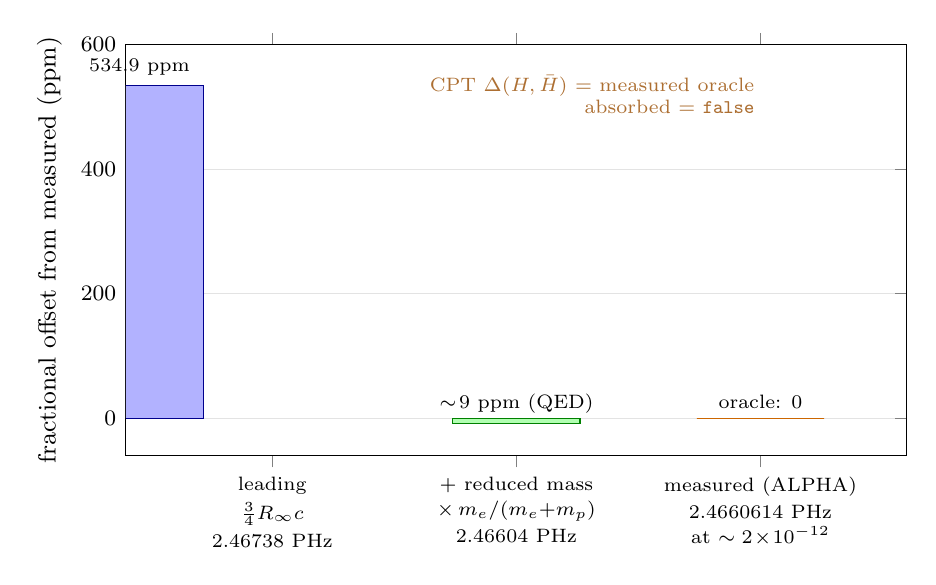
\begin{tikzpicture}
\begin{axis}[
  width=11.5cm, height=6.8cm,
  ybar,
  bar width=46pt,
  ymin=-60, ymax=600,
  ylabel={fractional offset from measured (ppm)},
  symbolic x coords={leading, reduced, measured},
  xtick={leading, reduced, measured},
  xticklabels={%
    \shortstack{leading\\\scriptsize $\frac34 R_\infty c$\\\scriptsize 2.46738 PHz},
    \shortstack{+ reduced mass\\\scriptsize $\times\,m_e/(m_e{+}m_p)$\\\scriptsize 2.46604 PHz},
    \shortstack{measured (ALPHA)\\\scriptsize 2.4660614 PHz\\\scriptsize at $\sim2\!\times\!10^{-12}$}},
  x tick label style={font=\scriptsize, align=center},
  tick label style={font=\footnotesize},
  label style={font=\small},
  nodes near coords,
  nodes near coords style={font=\scriptsize},
  point meta=explicit symbolic,
  ymajorgrids, grid style={gray!22},
  enlarge x limits=0.30,
]
\addplot[draw=blue!55!black, fill=blue!30] coordinates {
  (leading,  534.9) [534.9 ppm]
};
\addplot[draw=green!50!black, fill=green!30, bar shift=0pt] coordinates {
  (reduced,  -8.7)  [$\sim\!9$ ppm (QED)]
};
\addplot[draw=orange!80!black, fill=orange!30, bar shift=0pt] coordinates {
  (measured, 0)     [oracle: 0]
};
% honesty note
\node[font=\scriptsize, text=orange!60!black, anchor=north east, align=right,
  fill=white, fill opacity=0.8, inner sep=2pt]
  at (axis cs:measured, 560)
  {CPT $\Delta(H,\bar H)$ = measured oracle\\absorbed = \texttt{false}};
\end{axis}
\end{tikzpicture}
\end{document}
